%==============================================================================
% TEMPLATE LAPORAN AKHIR PROYEK PENGGANTI UAS
% Mata Kuliah Kecerdasan Buatan | Teknik Komputer - Universitas Indonesia
% Semester Genap 2025/2026
%
% Cara pakai:
%   1. Ganti seluruh teks yang ada di dalam [...] atau \TODO{...}.
%   2. Hapus blok "petunjuk" (yang ditandai dengan environment "petunjuk")
%      setelah subbab terkait selesai diisi.
%   3. Kompilasi dengan XeLaTeX (rekomendasi):
%        xelatex template-laporan-akhir.tex
%        xelatex template-laporan-akhir.tex    % run ke-2 untuk DaftarIsi/refs
%   4. Sitasi pakai BibTeX gaya IEEE (file referensi.bib).
%==============================================================================

\documentclass[11pt,a4paper,oneside]{report}

%------ Bahasa & Font --------------------------------------------------------
\usepackage{fontspec}
\setmainfont{Times New Roman}
\setmonofont{Consolas}[
  Path = fonts/,
  UprightFont = consola.ttf,
  BoldFont = consolab.ttf,
  ItalicFont = consolai.ttf,
  BoldItalicFont = consolaz.ttf,
  Scale = 0.92
]

%------ Geometri & Spasi -----------------------------------------------------
\usepackage[a4paper,margin=2.5cm]{geometry}
\usepackage{setspace}
\onehalfspacing
\setlength{\parskip}{0.5em}

%------ Paket Pendukung ------------------------------------------------------
\usepackage{graphicx}
\usepackage{amsmath,amssymb,amsfonts}
\usepackage{booktabs}
\usepackage{array}
\usepackage{tabularx}
\usepackage{longtable}
\usepackage{enumitem}
\usepackage{xcolor}
\usepackage{listings}
\usepackage{hyperref}
\usepackage{titlesec}
\usepackage{tcolorbox}
\usepackage{caption}
\usepackage{tikz}
\usetikzlibrary{shapes.geometric, arrows.meta, positioning, fit, backgrounds}
\usepackage[backend=biber,style=ieee]{biblatex}

%------ Penyesuaian Bahasa Indonesia (manual, tanpa babel) -------------------
\renewcommand{\chaptername}{BAB}
\renewcommand{\contentsname}{DAFTAR ISI}
\renewcommand{\listfigurename}{DAFTAR GAMBAR}
\renewcommand{\listtablename}{DAFTAR TABEL}
\renewcommand{\bibname}{DAFTAR PUSTAKA}
\renewcommand{\appendixname}{LAMPIRAN}
\renewcommand{\figurename}{Gambar}
\renewcommand{\tablename}{Tabel}

%------ Format Bab (BAB I, BAB II, ...) --------------------------------------
\titleformat{\chapter}[display]
  {\normalfont\Large\bfseries\centering}
  {\chaptername\ \thechapter}{12pt}{\Large}
\titlespacing*{\chapter}{0pt}{-20pt}{20pt}

%------ Hyperref -------------------------------------------------------------
\hypersetup{
  colorlinks=true,
  linkcolor=black,
  urlcolor=blue,
  citecolor=black,
  pdftitle={Laporan Akhir Proyek - MK Kecerdasan Buatan},
  pdfauthor={Kelompok K02}
}

%------ Box Petunjuk Pengisian (HAPUS setelah subbab terisi) ----------------
\newtcolorbox{petunjuk}{
  colback=yellow!10,
  colframe=orange!60!black,
  boxrule=0.5pt,
  arc=2pt,
  left=6pt,right=6pt,top=4pt,bottom=4pt,
  fontupper=\small\itshape
}

%------ Listing untuk JSON ---------------------------------------------------
\lstdefinelanguage{json}{
  basicstyle=\ttfamily\footnotesize,
  showstringspaces=false,
  breaklines=true,
  frame=single,
  rulecolor=\color{gray!50},
  string=[s]{"}{"},
  stringstyle=\color{blue!60!black},
  comment=[l]{//},
  commentstyle=\color{green!50!black}
}

%------ Bibliography (siapkan referensi.bib di folder yang sama) -------------
\addbibresource{referensi.bib}

%==============================================================================
\begin{document}

%==============================================================================
% HALAMAN SAMPUL
%==============================================================================
\begin{titlepage}
\centering
\vspace*{1cm}

{\Large\bfseries LAPORAN AKHIR \par}
{\large PROYEK PENGGANTI UAS \par}
\vspace{0.3cm}
{\large Mata Kuliah Kecerdasan Buatan \par}
{\large Semester Genap 2025/2026 \par}

\vspace{2cm}

% Logo opsional
% \includegraphics[width=0.25\textwidth]{logo-ui.png}

\vspace{1.5cm}

{\LARGE\bfseries VisionGuard \par}

\vspace{0.5cm}

{\large Sistem Pendeteksi Kelelahan Pengemudi Kendaraan dengan \textit{Convolutional Neural Network} \par}

\vspace{2cm}

{\large Disusun oleh: \par}

\vspace{0.5cm}

\begin{tabular}{rl}
Benedict Aurelius & 2306209095\\
Deandro Najwan Ahmad Syahbanna & 2306213174 \\
Nelson Laurensius & 2306161845 \\
Wesley Frederick Oh & 2306202763 \\
\end{tabular}

\vspace{1.5cm}

{\large Dosen Pengampu: \par}

{\large Muhammad Firdaus Syawaludin Lubis, S.T., M.T., Ph.D. \par}

\vfill

{\large DEPARTEMEN TEKNIK KOMPUTER \par}

{\large FAKULTAS TEKNIK \par}

{\large UNIVERSITAS INDONESIA \par}

{\large 2026 \par}
\end{titlepage}

%==============================================================================
% LEMBAR PERNYATAAN ORISINALITAS
%==============================================================================
\chapter*{LEMBAR PERNYATAAN ORISINALITAS}
\addcontentsline{toc}{chapter}{Lembar Pernyataan Orisinalitas}

Kami yang bertandatangan di bawah ini menyatakan bahwa laporan ini, beserta seluruh isinya (termasuk Sub-bab IV.x masing-masing anggota dan berkas \texttt{metadata.json} yang merupakan bagian tidak terpisahkan), adalah hasil karya kelompok kami sendiri. Setiap kutipan, kode, atau gambar yang berasal dari sumber lain telah disitasi dengan benar. Penggunaan AI \textit{assistant} telah dideklarasikan secara jujur pada Sub-bab IV.x.2.

\vspace{1.5cm}

\noindent
\begin{tabular}{p{0.45\textwidth}p{0.45\textwidth}}
\centering Benedict Aurelius & \centering Deandro Najwan Ahmad Syahbanna \tabularnewline
\centering NPM. 2306209095 & \centering NPM. 2306213174 \tabularnewline
\centering 
\includegraphics[height=2cm]{memberSign/benedict.jpeg} & \centering 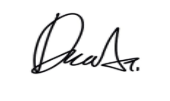
\includegraphics[height=2cm]{memberSign/TandaTangan_DeadnroNajwanAhmadSyahbanna.png} \tabularnewline
\centering (Benedict Aurelius) & \centering (Deandro Najwan Ahmad Syahbanna) \tabularnewline
\end{tabular}

\vspace{1cm}

\noindent
\begin{tabular}{p{0.45\textwidth}p{0.45\textwidth}}
\centering Nelson Laurensius & \centering Wesley Frederick Oh \tabularnewline
\centering NPM. 2306161845 & \centering NPM. 2306202763 \tabularnewline
\centering 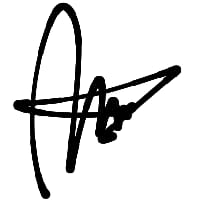
\includegraphics[height=2cm]{memberSign/nelson.jpeg} & \centering 
\includegraphics[height=2cm]{memberSign/wesley.jpeg} \tabularnewline
\centering (Nelson Laurensius) & \centering (Wesley Frederick Oh) \tabularnewline
\end{tabular}

%==============================================================================
% DAFTAR ISI, GAMBAR, TABEL
%==============================================================================
\tableofcontents
\listoffigures
\listoftables

%==============================================================================
% ABSTRAK
%==============================================================================
\chapter*{ABSTRAK}
\addcontentsline{toc}{chapter}{Abstrak}

Kecelakaan lalu lintas akibat kelelahan pengemudi merupakan permasalahan keselamatan publik yang signifikan, dengan 61\% dari 148.000 kecelakaan di Indonesia pada tahun 2023 disebabkan oleh faktor manusia. Proyek VisionGuard mengembangkan sistem pendeteksi kelelahan pengemudi (\textit{Driver Drowsiness Detection}) menggunakan arsitektur \textit{Faster Region-based Convolutional Neural Network} (Faster R-CNN) dengan \textit{backbone} ResNet-50 FPN. Berbeda dengan pendekatan klasifikasi gambar global yang umum digunakan, Faster R-CNN dipilih karena kemampuannya dalam melokalisasi posisi indikator kelelahan secara spasial melalui \textit{bounding box} sekaligus mengklasifikasikan kondisi pengemudi ke dalam empat kelas: \textit{Normal}, \textit{Yawning}, \textit{Sleepy Combination}, dan \textit{Slow Blink with Nodding}. Model dilatih dan dievaluasi menggunakan dataset NTHU-DDD \textit{Multi-class} yang terdiri dari 66.521 gambar dengan variasi pencahayaan (siang/malam), penggunaan kacamata, dan keragaman subjek. Pembagian dataset dilakukan dengan rasio 75:15:10 untuk \textit{training}, \textit{validation}, dan \textit{test set}. Dengan konfigurasi \textit{optimizer} SGD (\textit{learning rate} 0,005), \textit{batch size} 4, dan \textit{transfer learning} dari bobot COCO, model terbaik diperoleh pada Epoch ke-3 dengan mAP@[0.5:0.95] sebesar \textbf{0,8749} dan mAP@0.50 sebesar \textbf{0,9343} pada \textit{test set}. Performa per kelas menunjukkan skor mAP tertinggi pada kelas \texttt{sleepyCombination} (0,9175), diikuti \texttt{yawning} (0,8680), \texttt{slowBlinkWithNodding} (0,8572), dan \texttt{notdrowsy} (0,8568). Hasil ini menunjukkan bahwa pendekatan \textit{object detection} berbasis Faster R-CNN efektif dan menjanjikan untuk aplikasi sistem keselamatan berkendara.

\vspace{1em}
\noindent\textbf{Kata kunci:} \textit{Driver Drowsiness Detection}, Faster R-CNN, \textit{Convolutional Neural Network}, NTHU-DDD, \textit{Object Detection}

%==============================================================================
% BAB I - PENDAHULUAN & DEFINISI MASALAH
%==============================================================================
\chapter{PENDAHULUAN \& DEFINISI MASALAH}
\label{bab:pendahuluan}

\section{Topik yang Dipilih}

Topik yang dipilih pada proyek ini adalah \textbf{Topik 1: Convolutional Neural Network (CNN)}, yaitu pengembangan sistem berbasis \textit{deep learning} dengan arsitektur CNN untuk menyelesaikan permasalahan di domain \textit{computer vision}. Secara spesifik, proyek ini mengimplementasikan arsitektur \textit{Faster Region-based Convolutional Neural Network} (Faster R-CNN) \cite{ren2015faster} untuk membangun sistem pendeteksi kelelahan pengemudi kendaraan (\textit{Driver Drowsiness Detection}).

Pemilihan topik ini dilandasi oleh tiga pertimbangan utama. \textit{Pertama}, seluruh anggota tim memiliki latar belakang yang kuat di bidang Teknik Komputer dengan pengalaman dalam pengolahan citra digital dan pemrograman menggunakan \textit{framework} PyTorch, sehingga pengembangan model berbasis CNN merupakan domain yang sesuai dengan kompetensi kolektif tim. \textit{Kedua}, ketersediaan dataset publik berkualitas tinggi, yaitu NTHU Driver Drowsiness Detection (NTHU-DDD) \cite{weng2017driver} dari Kaggle, memungkinkan proses \textit{training} dan evaluasi model yang komprehensif tanpa kendala akuisisi data. \textit{Ketiga}, permasalahan kecelakaan lalu lintas akibat kelelahan pengemudi merupakan isu keselamatan publik yang sangat mendesak, khususnya di Indonesia, sehingga pengembangan solusi berbasis kecerdasan buatan pada domain ini memiliki dampak sosial yang signifikan dan aplikabilitas dunia nyata.

\section{Latar Belakang}

Penggunaan kendaraan pribadi, terutama di Indonesia, sangat populer dan menjadi alternatif utama dibandingkan kendaraan umum seperti kereta dan bus. Salah satu implikasinya adalah pesatnya pertumbuhan mobilitas perkotaan yang diiringi dengan meningkatnya risiko kecelakaan lalu lintas. Sebagian besar kecelakaan kendaraan darat ditimbulkan akibat \textit{human error}, di mana kelelahan pengemudi dan kekurangan tidur menjadi faktor dominan. Di Indonesia pada tahun 2023, dari 148.000 jumlah kecelakaan lalu lintas yang terjadi, 61\% di antaranya disebabkan oleh faktor manusia seperti mengantuk, ceroboh, dan kurang konsentrasi \cite{goodstats2023}. Pada daerah perkotaan yang padat kendaraan, kelalaian pengendara selama dua detik saja dapat menyebabkan kecelakaan yang sangat fatal.

Perkembangan dalam bidang \textit{computer vision} dan kecerdasan buatan sangat memungkinkan implementasi sistem \textit{camera-based Driver Drowsiness Detection} (DDD) \cite{deng2019deep, ed2020deep}. Namun, tantangan terbesar dalam aplikasi \textit{computer vision} untuk skenario berkendara adalah tingkat pencahayaan yang sangat bervariasi tergantung tempat dan waktu, penggunaan aksesoris wajah seperti kacamata atau kacamata hitam, serta fitur wajah yang sangat bervariasi tergantung etnis dan karakteristik individu \cite{abbas2024ddd}. Banyak model yang ada dilatih pada kumpulan data gambar statis sederhana yang gagal mereplikasi kompleksitas lingkungan dinamis sesungguhnya, sehingga menghasilkan tingkat kesalahan positif yang tinggi dalam penerapan praktis.

Untuk mengatasi permasalahan tersebut, proyek ini menggunakan dataset NTHU Driver Drowsiness Detection (NTHU-DDD) \cite{weng2017driver} yang secara khusus dirancang untuk merepresentasikan skenario berkendara di dunia nyata. Dataset ini mencakup berbagai variasi kondisi pencahayaan (siang dan malam), penggunaan aksesoris (kacamata dan kacamata hitam), serta keragaman subjek pengemudi. Lebih lanjut, mengklasifikasikan seluruh \textit{frame} gambar sebagai ``mengantuk'' atau ``sadar'' saja tidak memberikan presisi spasial yang dibutuhkan untuk sistem keselamatan yang dapat diaudit dan divalidasi \cite{ma2024hybrid}. Oleh karena itu, proyek ini mengusulkan implementasi arsitektur Faster R-CNN \cite{ren2015faster}. Dengan memanfaatkan \textit{Region Proposal Network} (RPN) terintegrasinya, Faster R-CNN unggul dalam melokalisasi titik-titik fokus indikator kelelahan secara presisi seperti koordinat tepat mata yang terkulai atau mulut yang menguap dalam konteks latar belakang kabin kendaraan. Hal ini memastikan bahwa prediksi kantuk terkait erat dengan fitur wajah pengemudi yang sebenarnya, menghasilkan alur deteksi yang akurat dan transparan.

\section{Rumusan Masalah}

Berdasarkan latar belakang yang telah diuraikan, rumusan masalah pada proyek ini dirumuskan sebagai berikut:

\begin{enumerate}[label=RM\arabic*.,leftmargin=*]
    \item {Sejauh mana arsitektur Faster R-CNN dengan \textit{backbone} ResNet-50 FPN mampu melokalisasi dan mengklasifikasikan indikator kelelahan pengemudi (\textit{yawning}, \textit{slow blinking/sleeping}, \textit{nodding}, dan \textit{normal}) secara akurat menggunakan dataset NTHU-DDD, yang diukur melalui metrik mAP@[0.5:0.95]?}
    \item {Bagaimana ketahanan (\textit{robustness}) model Faster R-CNN dalam mendeteksi kelelahan pengemudi ketika dihadapkan pada variasi kondisi dunia nyata, meliputi perubahan pencahayaan (siang/malam), penggunaan kacamata, serta keragaman karakteristik wajah subjek?}
    \item {Apakah pendekatan \textit{object detection} berbasis Faster R-CNN memberikan keunggulan signifikan dibandingkan metode \textit{global image classification} konvensional dalam hal presisi lokalisasi spasial dan transparansi proses pengambilan keputusan untuk sistem keselamatan berkendara?}
\end{enumerate}

\section{Tujuan Proyek}

Sejalan dengan rumusan masalah di atas, proyek ini memiliki tujuan-tujuan berikut:

\begin{enumerate}[label=T\arabic*.,leftmargin=*]
    \item {Menerapkan arsitektur Faster R-CNN dengan \textit{backbone} ResNet-50 FPN dan \textit{pre-trained weights} COCO untuk membangun sistem \textit{Driver Drowsiness Detection} yang mampu melokalisasi dan mengklasifikasikan empat kelas indikator kelelahan pengemudi secara simultan. (\textit{Terkait RM1})}
    \item {Mengevaluasi performa kuantitatif model menggunakan metrik \textit{Mean Average Precision} (mAP) pada \textit{test set} yang mencakup berbagai variasi kondisi pencahayaan dan aksesoris wajah, guna mengukur tingkat ketahanan model terhadap kondisi dunia nyata. (\textit{Terkait RM2})}
    \item {Menganalisis akurasi lokalisasi spasial \textit{bounding box} model dalam mendeteksi \textit{Region of Interest} (RoI) pada area wajah, mata, dan mulut pengemudi, beserta transparansi keputusan klasifikasi yang dihasilkan. (\textit{Terkait RM3})}
    \item {Membangun \textit{inference pipeline} operasional yang mampu memproses input gambar dan menghasilkan prediksi deteksi kantuk secara visual, guna mendemonstrasikan kelayakan dan aplikabilitas praktis arsitektur yang diusulkan. (\textit{Terkait RM1 \& RM3})}
\end{enumerate}

\section{Ruang Lingkup \& Batasan}

Ruang lingkup proyek ini didefinisikan pada beberapa dimensi berikut:

\begin{itemize}[leftmargin=*]
    \item \textbf{Domain Data.} Proyek ini menggunakan dataset publik NTHU-DDD \textit{Multi-class} dari Kaggle yang berisi 66.521 \textit{frame} gambar (\texttt{.jpg}) dengan resolusi $640 \times 640$ piksel. Dataset mencakup variasi pencahayaan (siang dan malam/inframerah), penggunaan kacamata (tanpa kacamata, kacamata biasa, kacamata hitam), serta keragaman subjek pengemudi.
    \item \textbf{Kelas Target.} Klasifikasi dilakukan terhadap empat kelas indikator perilaku pengemudi, yaitu: \textit{Normal/Not Drowsy}, \textit{Yawning} (menguap), \textit{Sleepy Combination} (mata tertutup/\textit{micro sleep}), dan \textit{Slow Blink with Nodding} (kedipan lambat dengan anggukan kepala).
    \item \textbf{Arsitektur Model.} Model yang digunakan adalah Faster R-CNN dengan \textit{backbone} ResNet-50 FPN yang di-\textit{fine-tune} dari bobot \textit{pre-trained} COCO (\texttt{fasterrcnn\_resnet50\_fpn}).
    \item \textbf{Metrik Evaluasi.} Evaluasi performa difokuskan pada metrik \textit{Mean Average Precision} (mAP) standar pada \textit{object detection}, yaitu mAP@[0.5:0.95] dan mAP@0.50. Metrik tambahan meliputi \textit{Precision}, \textit{Recall}, dan \textit{Confusion Matrix} per kelas.
\end{itemize}

\noindent Adapun batasan-batasan yang secara eksplisit \textbf{tidak} dikerjakan dalam proyek ini adalah sebagai berikut:

\begin{itemize}[leftmargin=*]
    \item Proyek ini \textbf{tidak} melakukan eksplorasi arsitektur \textit{backbone} alternatif (seperti VGG-16, ResNet-101, atau Vision Transformer/ViT) dan hanya menggunakan satu varian \textit{backbone}, yaitu ResNet-50 FPN.
    \item Proyek ini \textbf{tidak} mengimplementasikan analisis temporal (\textit{sequence-based detection}) menggunakan arsitektur RNN/LSTM. Model beroperasi pada \textit{single-frame detection} tanpa mempertimbangkan konteks antar-\textit{frame} secara sekuensial.
    \item Proyek ini \textbf{tidak} melakukan evaluasi pada dataset \textit{out-of-distribution} selain NTHU-DDD (misalnya YAWDD atau UTA-RLDD) untuk menguji generalisasi lintas dataset.
    \item Proyek ini \textbf{tidak} melakukan \textit{hyperparameter tuning} secara ekstensif menggunakan metode pencarian otomatis (\textit{grid search}, \textit{random search}, atau \textit{Bayesian optimization}). Konfigurasi \textit{hyperparameter} ditetapkan berdasarkan praktik terbaik dari literatur.
    \item Proyek ini \textbf{tidak} melakukan \textit{deployment} pada perangkat \textit{edge} (\textit{embedded system}) di dalam kendaraan. Demonstrasi \textit{inference} dilakukan pada lingkungan Google Colab.
\end{itemize}

%==============================================================================
% BAB II - PENDEKATAN AI
%==============================================================================
\chapter{PENDEKATAN AI}
\label{bab:pendekatan}

\section{Tinjauan Pustaka (\textit{Related Work})}

Penelitian mengenai deteksi kelelahan pengemudi berbasis \textit{computer vision} telah berkembang pesat dalam beberapa tahun terakhir. Tabel~\ref{tab:related-work} merangkum lima studi terpenting yang menjadi landasan dan pembanding bagi proyek ini.

\begin{table}[h!]
\centering
\caption{Ringkasan tinjauan pustaka}
\label{tab:related-work}
\footnotesize
\begin{tabularx}{\textwidth}{p{2.2cm}XXXX}
\toprule
\textbf{Penulis (Th.)} & \textbf{Metode} & \textbf{Dataset} & \textbf{Hasil} & \textbf{Keterbatasan} \\
\midrule
Weng et al. (2017) \cite{weng2017driver} & Hierarchical Temporal Deep Belief Network & NTHU-DDD & Akurasi klasifikasi 85\% pada multi-skenario & Tidak melokalisasi area wajah; klasifikasi \textit{frame}-level \\
Deng \& Wu (2019) \cite{deng2019deep} & CNN + Facial Landmarks (EAR/MAR) & Dataset kustom & Akurasi 94.2\% & Sensitif terhadap oklusi wajah; dataset terbatas \\
Ed-Doughmi et al. (2020) \cite{ed2020deep} & CNN + RNN (temporal) & NTHU-DDD & Akurasi 90\% & Kompleksitas komputasi tinggi; latensi tidak cocok untuk \textit{real-time} \\
Ma et al. (2024) \cite{ma2024hybrid} & Hybrid YOLOv5s + Faster R-CNN & Custom road-scene & mAP 78.3\% & Fokus pada objek jalan, bukan spesifik wajah pengemudi \\
Abbas \& Alsheddy (2024) \cite{abbas2024ddd} & Survey multi-sensor DDD & Multi-dataset & Review sistematis & Tidak mengusulkan arsitektur baru; hanya komparasi \\
\bottomrule
\end{tabularx}
\end{table}

Berdasarkan tinjauan literatur di atas, mayoritas studi yang ada menggunakan pendekatan \textit{global image classification} yang mengklasifikasikan seluruh \textit{frame} tanpa melokalisasi area spesifik pada wajah, atau menggunakan metode \textit{facial landmark} yang memerlukan tahap pra-pemrosesan terpisah. Proyek VisionGuard ini memposisikan diri sebagai pendekatan yang \textbf{mengintegrasikan lokalisasi spasial dan klasifikasi secara simultan} melalui arsitektur Faster R-CNN, sehingga menghasilkan prediksi yang tidak hanya akurat secara klasifikasi tetapi juga transparan dan dapat diaudit melalui koordinat \textit{bounding box} yang eksplisit.

\section{Landasan Teori Model yang Dipilih}

Pendekatan kecerdasan buatan yang digunakan dalam proyek ini berpusat pada arsitektur \textit{Faster Region-based Convolutional Neural Network} (Faster R-CNN), yang diperkenalkan oleh Ren et al. \cite{ren2015faster}. Faster R-CNN merupakan arsitektur \textit{two-stage object detector} yang memiliki keunggulan performa akurasi tinggi dalam melokalisasi posisi objek dan mengenali kelas secara simultan.

\subsection{Operasi Konvolusi pada CNN}

Fondasi dari seluruh arsitektur Faster R-CNN adalah operasi konvolusi yang mengekstraksi fitur dari citra input. Secara matematis, operasi konvolusi diskrit dua dimensi pada citra input $I$ dengan \textit{kernel/filter} $K$ berukuran $m \times n$ didefinisikan sebagai berikut:

\begin{equation}
\label{eq:konvolusi}
(I * K)(x, y) = \sum_{i=0}^{m-1} \sum_{j=0}^{n-1} I(x+i,\; y+j) \cdot K(i,\; j)
\end{equation}

\noindent dengan $I(x+i, y+j)$ adalah nilai intensitas piksel pada posisi $(x+i, y+j)$ dari citra input, $K(i,j)$ adalah bobot \textit{kernel} pada posisi $(i,j)$, dan $(x,y)$ adalah posisi spasial pada \textit{feature map} keluaran. Operasi ini diterapkan secara bertingkat (\textit{hierarchical}) pada setiap lapisan konvolusi untuk mengekstraksi fitur dari level rendah (tepi, tekstur) hingga level tinggi (bentuk mata, bibir).

\subsection{Backbone Network: ResNet-50 dengan FPN}

Komponen pertama Faster R-CNN bertugas sebagai pengekstrak fitur (\textit{feature extractor}). Pada proyek ini, \textit{backbone} yang digunakan adalah ResNet-50 \cite{he2016deep} yang dilengkapi dengan \textit{Feature Pyramid Network} (FPN) \cite{lin2017feature}. ResNet-50 memperkenalkan koneksi residual (\textit{skip connection}) yang memungkinkan pelatihan jaringan sangat dalam tanpa degradasi performa. FPN membangun piramida fitur multi-skala dari \textit{feature map} ResNet, sehingga model mampu mendeteksi objek pada berbagai ukuran secara efektif. Bobot awal (\textit{pre-trained weights}) diambil dari model yang telah dilatih pada dataset COCO \cite{lin2014coco} melalui mekanisme \textit{transfer learning}.

\subsection{Region Proposal Network (RPN)}

RPN merupakan inovasi inti yang membedakan Faster R-CNN dari pendahulunya \cite{girshick2015fast}. RPN memindai \textit{feature map} menggunakan mekanisme \textit{sliding window} dan menghasilkan kandidat kotak pembatas yang disebut \textit{Anchor Boxes} dengan berbagai variasi skala dan rasio aspek. RPN menghasilkan dua jenis \textit{output}:

\begin{itemize}[leftmargin=*]
    \item \textbf{\textit{Objectness Score}:} Skor probabilitas apakah \textit{anchor box} berisi objek atau latar belakang.
    \item \textbf{\textit{Bounding Box Regression}:} Koordinat penyesuaian posisi \textit{anchor box} agar lebih presisi membungkus objek target.
\end{itemize}

\subsection{RoI Pooling/Align dan Classification Head}

Kandidat RoI dari RPN memiliki dimensi bervariasi, sementara lapisan \textit{Fully Connected} (FC) memerlukan input berukuran tetap. \textit{RoI Align} menjembatani perbedaan ini melalui interpolasi bilinear. Hasil \textit{pooling} kemudian diproses oleh dua cabang output: (1) \textit{Softmax Classifier} untuk menentukan kelas objek (\textit{Normal}, \textit{Yawning}, \textit{Sleepy Combination}, atau \textit{Slow Blink with Nodding}), dan (2) \textit{Bounding Box Regressor} untuk menyempurnakan koordinat akhir $(x, y, w, h)$.

\subsection{Diagram Arsitektur}

Gambar~\ref{fig:arsitektur} mengilustrasikan alur pemrosesan citra pengemudi di dalam arsitektur Faster R-CNN yang digunakan pada proyek ini.

\begin{figure}[h!]
\centering
\resizebox{\textwidth}{!}{%
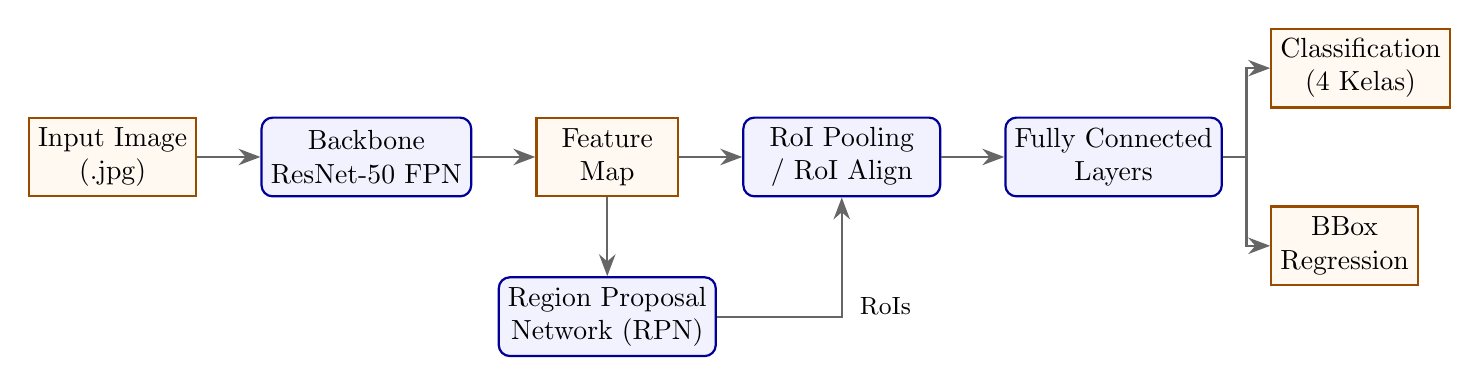
\begin{tikzpicture}[
    node distance=1cm and 0.8cm,
    box/.style={rectangle, draw=blue!60!black, fill=blue!5, thick, minimum width=2.5cm, minimum height=1cm, align=center, rounded corners},
    io/.style={rectangle, draw=orange!60!black, fill=orange!5, thick, minimum width=1.8cm, minimum height=1cm, align=center},
    arrow/.style={-{Stealth[scale=1.2]}, thick, draw=gray!80!black}
]
\node (input) [io] {Input Image\\(.jpg)};
\node (backbone) [box, right=of input] {Backbone\\ResNet-50 FPN};
\node (featuremap) [io, right=of backbone] {Feature\\Map};
\node (roi) [box, right=of featuremap] {RoI Pooling\\/ RoI Align};
\node (fc) [box, right=of roi] {Fully Connected\\Layers};
\node (rpn) [box, below=of featuremap] {Region Proposal\\Network (RPN)};
\node (class) [io, above right=0.1cm and 0.6cm of fc] {Classification\\(4 Kelas)};
\node (bbox) [io, below right=0.1cm and 0.6cm of fc] {BBox\\Regression};
\draw [arrow] (input) -- (backbone);
\draw [arrow] (backbone) -- (featuremap);
\draw [arrow] (featuremap) -- (roi);
\draw [arrow] (featuremap) -- (rpn);
\draw [arrow] (rpn.east) -| node[anchor=south west, xshift=0.1cm, yshift=-0.1cm] {\small RoIs} (roi.south);
\draw [arrow] (roi) -- (fc);
\draw [arrow] (fc.east) -- ++(0.3,0) |- (class.west);
\draw [arrow] (fc.east) -- ++(0.3,0) |- (bbox.west);
\end{tikzpicture}%
}
\caption{Diagram arsitektur Faster R-CNN untuk deteksi kantuk pengemudi (diadaptasi dari Ren et al. \cite{ren2015faster})}
\label{fig:arsitektur}
\end{figure}

\section{Justifikasi Ilmiah Pemilihan Pendekatan AI}

Pemilihan Faster R-CNN sebagai arsitektur utama didasarkan pada tiga pertimbangan ilmiah berikut:

\textbf{(1) Mengapa Faster R-CNN, bukan \textit{single-stage detector} (YOLO)?}
Arsitektur \textit{single-stage} seperti YOLO \cite{redmon2016yolo} memang unggul dalam kecepatan inferensi, namun cenderung kurang presisi dalam melokalisasi objek berukuran kecil dan objek yang saling berdekatan. Dalam konteks DDD, area wajah pengemudi seringkali mengandung beberapa indikator kelelahan yang berdekatan secara spasial (mata dan mulut), sehingga arsitektur \textit{two-stage} dengan RPN memberikan presisi lokalisasi yang lebih tinggi hal yang krusial untuk sistem keselamatan.

\textbf{(2) Mengapa bukan \textit{global image classifier} (ResNet/VGG biasa)?}
Pendekatan klasifikasi gambar utuh hanya menghasilkan label kelas tanpa informasi spasial tentang \textit{di mana} indikator kelelahan terdeteksi. Faster R-CNN menghasilkan \textit{bounding box} yang eksplisit, memberikan transparansi dan kemampuan audit yang dibutuhkan dalam sistem keselamatan berkendara.

\textbf{(3) \textit{Tradeoff} yang dipertimbangkan.}
Faster R-CNN memiliki \textit{tradeoff} berupa waktu inferensi yang lebih lambat dibandingkan YOLO ($\sim$5--7 FPS vs $\sim$30+ FPS). Namun, mengingat proyek ini memprioritaskan \textbf{akurasi deteksi dan presisi lokalisasi} di atas kecepatan \textit{real-time}, serta memanfaatkan \textit{transfer learning} dari bobot COCO yang mempercepat konvergensi \textit{training}, Faster R-CNN merupakan pilihan yang optimal. Ketersediaan dataset NTHU-DDD yang besar (66.521 gambar) juga memadai untuk melatih arsitektur \textit{two-stage} yang cenderung membutuhkan lebih banyak data dibandingkan \textit{single-stage}.

\section{\textit{Block Diagram} Sistem End-to-End}

Gambar~\ref{fig:block-diagram} menunjukkan alur kerja sistem VisionGuard secara menyeluruh, mulai dari data mentah hingga output prediksi deteksi kantuk.

\begin{figure}[h!]
\centering
\resizebox{\textwidth}{!}{%
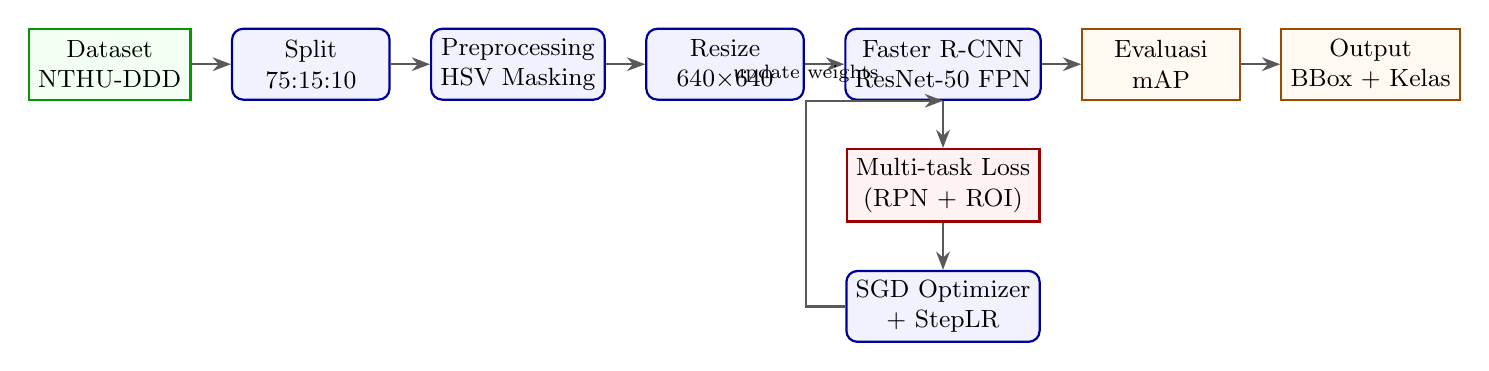
\begin{tikzpicture}[
    node distance=0.6cm and 0.5cm,
    block/.style={rectangle, draw=blue!60!black, fill=blue!5, thick, minimum width=2cm, minimum height=0.9cm, align=center, rounded corners, font=\small},
    data/.style={rectangle, draw=green!60!black, fill=green!5, thick, minimum width=2cm, minimum height=0.9cm, align=center, font=\small},
    loss/.style={rectangle, draw=red!60!black, fill=red!5, thick, minimum width=2cm, minimum height=0.9cm, align=center, font=\small},
    output/.style={rectangle, draw=orange!60!black, fill=orange!5, thick, minimum width=2cm, minimum height=0.9cm, align=center, font=\small},
    arrow/.style={-{Stealth[scale=1]}, thick, draw=gray!70!black}
]
\node (dataset) [data] {Dataset\\NTHU-DDD};
\node (split) [block, right=of dataset] {Split\\75:15:10};
\node (preprocess) [block, right=of split] {Preprocessing\\HSV Masking};
\node (augment) [block, right=of preprocess] {Resize\\640$\times$640};
\node (model) [block, right=of augment] {Faster R-CNN\\ResNet-50 FPN};
\node (loss) [loss, below=of model] {Multi-task Loss\\(RPN + ROI)};
\node (optimizer) [block, below=of loss] {SGD Optimizer\\+ StepLR};
\node (eval) [output, right=of model] {Evaluasi\\mAP};
\node (out) [output, right=of eval] {Output\\BBox + Kelas};
\draw [arrow] (dataset) -- (split);
\draw [arrow] (split) -- (preprocess);
\draw [arrow] (preprocess) -- (augment);
\draw [arrow] (augment) -- (model);
\draw [arrow] (model) -- (eval);
\draw [arrow] (eval) -- (out);
\draw [arrow] (model) -- (loss);
\draw [arrow] (loss) -- (optimizer);
\draw [arrow] (optimizer.west) -- ++(-0.5,0) |- node[anchor=south, yshift=0.1cm] {\scriptsize update weights} (model.south);
\end{tikzpicture}%
}
\caption{Block diagram sistem VisionGuard end-to-end}
\label{fig:block-diagram}
\end{figure}

\section{\textit{Flowchart} Program}

Gambar~\ref{fig:flowchart} menyajikan alur runtime program yang mencakup fase \textit{training} dan \textit{inference}.

\begin{figure}[h!]
\centering
\resizebox{0.85\textwidth}{!}{%
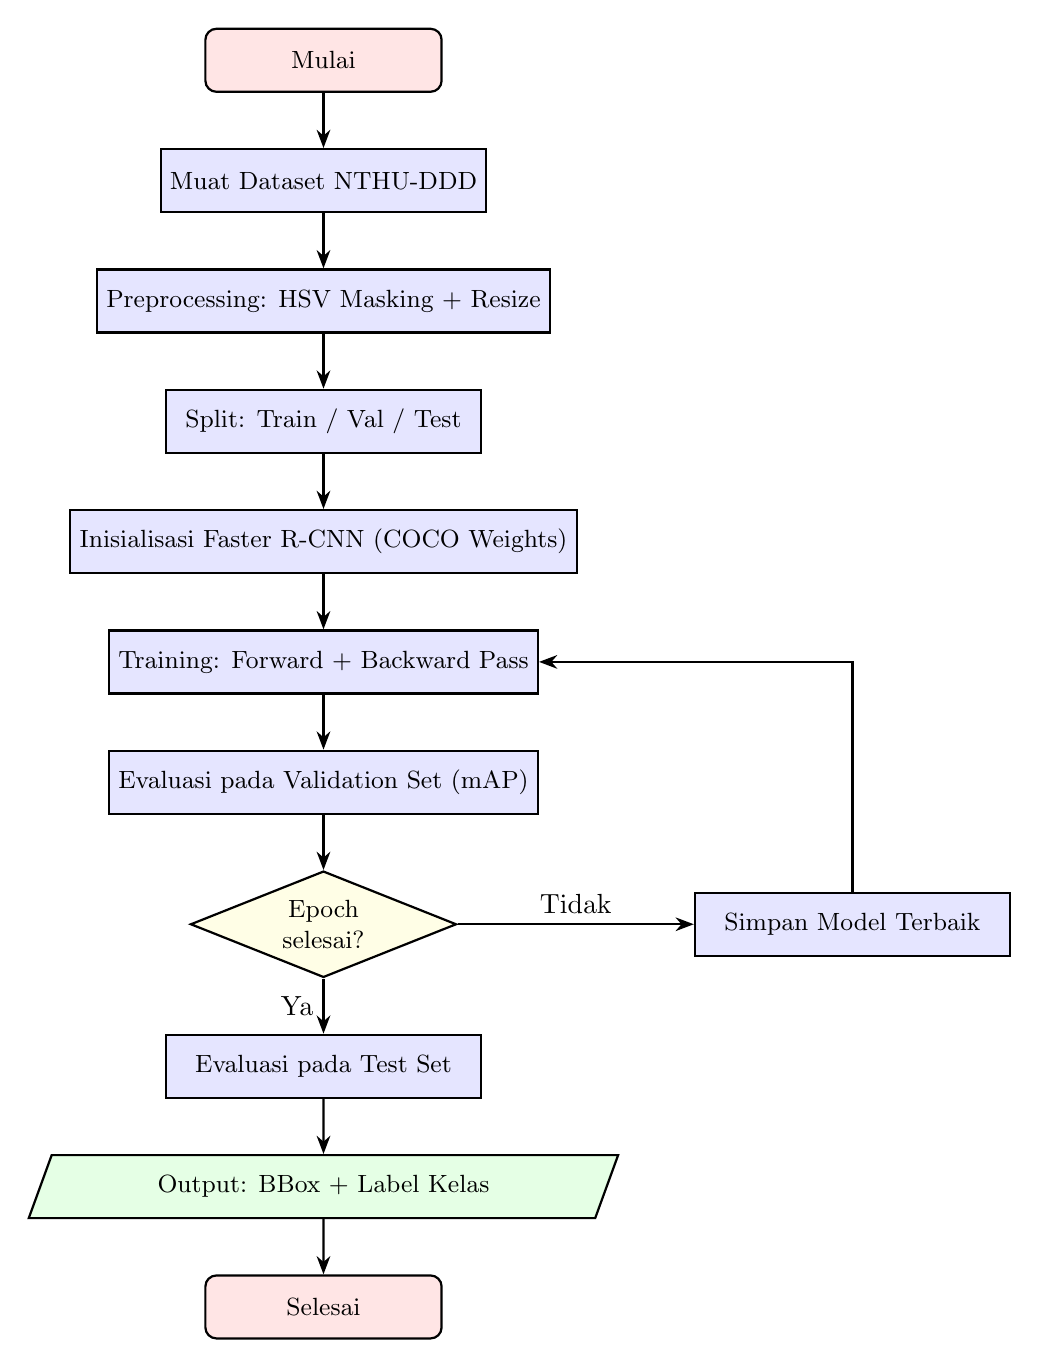
\begin{tikzpicture}[
    node distance=0.7cm,
    startstop/.style={rectangle, rounded corners, draw=black, fill=red!10, thick, minimum width=3cm, minimum height=0.8cm, align=center, font=\small},
    process/.style={rectangle, draw=black, fill=blue!10, thick, minimum width=4cm, minimum height=0.8cm, align=center, font=\small},
    decision/.style={diamond, draw=black, fill=yellow!10, thick, minimum width=2.5cm, minimum height=1cm, align=center, font=\small, aspect=2.5},
    io/.style={trapezium, trapezium left angle=70, trapezium right angle=110, draw=black, fill=green!10, thick, minimum width=3cm, minimum height=0.8cm, align=center, font=\small},
    arrow/.style={-{Stealth[scale=1]}, thick}
]
\node (start) [startstop] {Mulai};
\node (load) [process, below=of start] {Muat Dataset NTHU-DDD};
\node (preprocess) [process, below=of load] {Preprocessing: HSV Masking + Resize};
\node (split) [process, below=of preprocess] {Split: Train / Val / Test};
\node (initmodel) [process, below=of split] {Inisialisasi Faster R-CNN (COCO Weights)};
\node (train) [process, below=of initmodel] {Training: Forward + Backward Pass};
\node (evalval) [process, below=of train] {Evaluasi pada Validation Set (mAP)};
\node (checkepoch) [decision, below=of evalval] {Epoch\\selesai?};
\node (savebest) [process, right=3cm of checkepoch] {Simpan Model Terbaik};
\node (evaltest) [process, below=of checkepoch] {Evaluasi pada Test Set};
\node (inference) [io, below=of evaltest] {Output: BBox + Label Kelas};
\node (stop) [startstop, below=of inference] {Selesai};
\draw [arrow] (start) -- (load);
\draw [arrow] (load) -- (preprocess);
\draw [arrow] (preprocess) -- (split);
\draw [arrow] (split) -- (initmodel);
\draw [arrow] (initmodel) -- (train);
\draw [arrow] (train) -- (evalval);
\draw [arrow] (evalval) -- (checkepoch);
\draw [arrow] (checkepoch) -- node[anchor=south] {Tidak} (savebest);
\draw [arrow] (savebest.north) |- (train.east);
\draw [arrow] (checkepoch) -- node[anchor=east] {Ya} (evaltest);
\draw [arrow] (evaltest) -- (inference);
\draw [arrow] (inference) -- (stop);
\end{tikzpicture}%
}
\caption{Flowchart program \textit{training} dan \textit{inference} VisionGuard}
\label{fig:flowchart}
\end{figure}

%==============================================================================
% BAB III - IMPLEMENTASI & HASIL EKSPERIMEN
%==============================================================================
\chapter{IMPLEMENTASI \& HASIL EKSPERIMEN}
\label{bab:implementasi}

\section{Dataset \& Pra-pemrosesan}

\begin{sloppypar}
Pada eksperimen ini, dataset yang digunakan adalah \textit{National Tsing Hua University Driver Drowsiness Detection} (NTHU-DDD) \textit{Multi-Class} yang diperoleh dari repositori publik Kaggle \cite{weng2017driver}. NTHU-DDD merupakan salah satu dataset tolok ukur (\textit{benchmark}) standar yang diakui secara luas untuk melatih dan mengevaluasi model \textit{computer vision} dalam mendeteksi kelelahan pengemudi. Dataset ini memiliki total 66.521 gambar berformat \texttt{.jpg} yang terbagi ke dalam 4 kelas objek perilaku pengemudi: \texttt{notdrowsy} (30.491 gambar), \texttt{sleepyCombination} (17.756 gambar), \texttt{slowBlinkWithNodding} (9.412 gambar), dan \texttt{yawning} (8.862 gambar).

Dataset ini dirancang secara khusus untuk merepresentasikan skenario berkendara di dunia nyata yang kompleks, dengan variasi meliputi: (1) kondisi pencahayaan siang hari dan malam hari (inframerah/NIR); (2) penggunaan aksesoris berupa kacamata biasa, kacamata hitam, dan tanpa kacamata; serta (3) keragaman subjek pengemudi dari berbagai karakteristik wajah.

Gambar \ref{fig:contoh-dataset} memperlihatkan tiga contoh sampel \textit{image} dari kelas yang berbeda yang digunakan dalam \textit{training}.

\begin{figure}[!ht]
\centering

\begin{minipage}{0.28\textwidth}
\centering
\fbox{
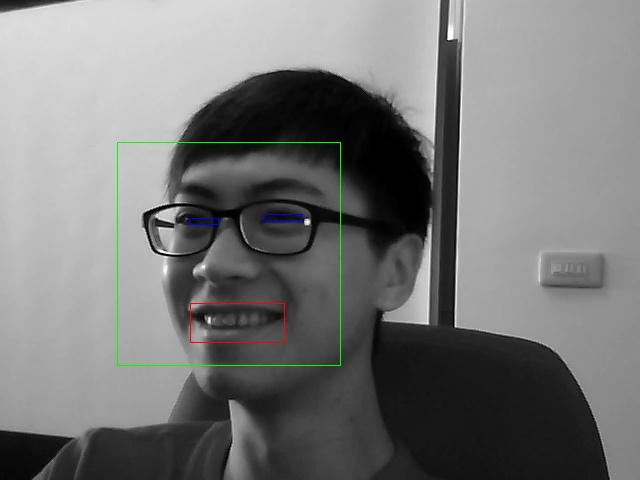
\includegraphics[
    width=0.95\linewidth,
    height=3cm,
    keepaspectratio
    ]{images/001_glasses_nonsleepyCombination_1014_notdrowsy.jpg}
}
\caption*{a) \texttt{notdrowsy}}
\end{minipage}
\hfill
\begin{minipage}{0.28\textwidth}
\centering
\fbox{
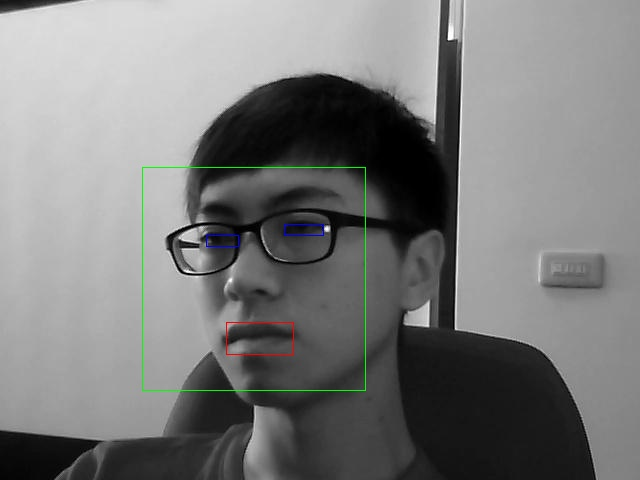
\includegraphics[
    width=0.95\linewidth,
    height=3cm,
    keepaspectratio
    ]{images/001_glasses_sleepyCombination_1002_drowsy.jpg}
}
\caption*{b) \texttt{sleepyCombination}}
\end{minipage}
\hfill
\begin{minipage}{0.28\textwidth}
\centering
\fbox{
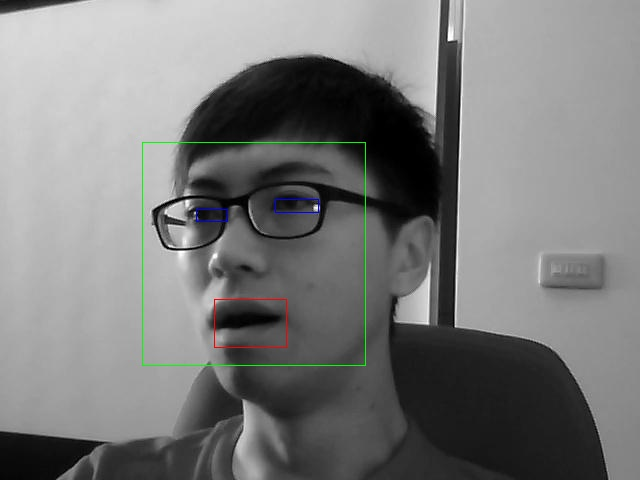
\includegraphics[
    width=0.95\linewidth,
    height=3cm,
    keepaspectratio
    ]{images/001_glasses_yawning_1001_drowsy.jpg}
}
\caption*{c) \texttt{yawning}}
\end{minipage}

\caption{Contoh 3 sampel dataset NTHU-DDD dari kelas yang berbeda}
\label{fig:contoh-dataset}

\end{figure}

Langkah \textit{pre-processing} yang dilakukan adalah ekstraksi \textit{bounding box} otomatis menggunakan teknik \textit{HSV Masking}. Karena posisi wajah pengemudi pada dataset ditandai dengan kotak berwarna (hijau, merah, atau biru), \textit{masking} dilakukan untuk mengambil koordinat ujung (x1, y1, x2, y2) dari kotak tersebut. Gambar kemudian diubah ukurannya (\textit{resize}) menjadi resolusi $640 \times 640$ piksel. Pembagian data dilakukan dengan proporsi 75\% untuk \textit{training}, 15\% untuk \textit{validation}, dan 10\% untuk \textit{testing}. Untuk memastikan hasil yang konsisten saat diulang, \textit{random seed} diatur pada nilai 42.

\end{sloppypar} %

% \begin{table}[htbp]
% \centering
% \caption{Pembagian dataset}
% \label{tab:split-data}
% \begin{tabular}{lrr}
% \toprule
% \textbf{Subset} & \textbf{Jumlah Sampel} & \textbf{Rasio (\%)} \\
% \midrule
% Training   & 49.890 & 75\% \\
% Validation & 9.978 & 15\% \\
% Test       & 6.653 & 10\% \\
% \midrule
% \textbf{Total} & \textbf{66.521} & \textbf{100\%} \\
% \bottomrule
% \end{tabular}
% \end{table}

\begin{center}
\captionof{table}{Pembagian dataset} 
\label{tab:split-data}
\begin{tabular}{lrr}
\toprule
\textbf{Subset} & \textbf{Jumlah Sampel} & \textbf{Rasio (\%)} \\
\midrule
Training   & 49.890 & 75\% \\
Validation & 9.978 & 15\% \\
Test       & 6.653 & 10\% \\
\midrule
\textbf{Total} & \textbf{66.521} & \textbf{100\%} \\
\bottomrule
\end{tabular}
\end{center} %


\section{Konfigurasi Eksperimen}

Sistem \textit{Vision Guard} dilatih menggunakan arsitektur Faster R-CNN dengan \textit{backbone} ResNet-50 FPN dan bobot awal (\textit{pre-trained weights}) dari dataset COCO. Lingkungan eksperimen dijalankan menggunakan \textit{framework} PyTorch dan Torchvision pada Google Colab menggunakan GPU Tesla T4 (VRAM 15.6 GB). Tabel \ref{tab:hyperparam} menyajikan nilai \textit{hyperparameter} yang digunakan selama proses pembuatan model. \textit{Library} tambahan yang digunakan meliputi OpenCV (v4.10) untuk pemrosesan gambar dan Albumentations (v1.4) untuk \textit{data augmentation}.

\begin{table}[h!]
\centering
\caption{Hyperparameter eksperimen}
\label{tab:hyperparam}
\begin{tabular}{ll}
\toprule
\textbf{Hyperparameter} & \textbf{Nilai} \\
\midrule
Arsitektur Model & Faster R-CNN (ResNet-50 FPN) \\
Learning rate    & 0.005 \\
Batch size       & 4 \\
Epoch Maksimal   & 20 \\
Optimizer        & SGD (Momentum = 0.9, Weight Decay = $5\times10^{-4}$) \\
Scheduler        & StepLR (Step Size = 7, Gamma = 0.1) \\
Score Threshold  & 0.5 \\
NMS Threshold    & 0.4 \\
Random seed      & 42 \\
\bottomrule
\end{tabular}
\end{table}

\section{Metrik Evaluasi}

Metrik evaluasi yang digunakan adalah \textit{Mean Average Precision} (mAP) yang dihitung menggunakan \textit{library} \texttt{torchmetrics}. mAP dipilih karena merupakan metrik standar untuk tugas \textit{object detection} yang mengukur akurasi klasifikasi kelas perilaku sekaligus mengukur seberapa akurat posisi \textit{bounding box} yang diprediksi dibandingkan dengan \textit{ground truth} melalui perhitungan \textit{Intersection over Union} (IoU). Evaluasi difokuskan pada dua varian:

\begin{itemize}[leftmargin=*]
    \item \textbf{mAP@0.50:} mAP pada \textit{IoU threshold} tunggal sebesar 0,50, yang mengukur akurasi deteksi dengan toleransi lokalisasi yang lebih longgar.
    \item \textbf{mAP@[0.5:0.95]:} mAP rata-rata pada rentang \textit{IoU threshold} dari 0,50 hingga 0,95 (dengan \textit{step} 0,05), yang merupakan metrik yang lebih ketat dan standar pada kompetisi \textit{object detection} seperti COCO.
\end{itemize}

Pemilihan mAP dibandingkan metrik klasifikasi biasa (akurasi, F1-score) didasarkan pada kebutuhan untuk mengevaluasi \textbf{lokalisasi spasial} dan \textbf{klasifikasi} secara bersamaan, yang merupakan karakteristik utama dari tugas \textit{object detection}.

\section{Hasil Kuantitatif}

Eksperimen menunjukkan bahwa proses \textit{training} model berjalan dengan baik. Evaluasi dilakukan pada setiap \textit{epoch} terhadap \textit{validation set}. Model terbaik didapatkan pada Epoch ke-3 dengan nilai mAP \textit{validation} sebesar 0.8785. Ketika model terbaik ini diuji menggunakan \textit{Test Set} (6.653 gambar), model menghasilkan nilai mAP@0.5:0.95 sebesar 0.8749 dan mAP@0.50 sebesar 0.9343.

\begin{table}[h!]
\centering
\caption{Hasil kuantitatif model (Metrik: mAP@[0.5:0.95])}
\label{tab:hasil}
\begin{tabular}{lcc}
\toprule
\textbf{Konfigurasi} & \textbf{Validation} & \textbf{Test} \\
\midrule
Epoch 1     & 0,8148 & -- \\
Epoch 2     & 0,8070 & -- \\
\textbf{Epoch 3 (Best Model)} & \textbf{0,8785} & \textbf{0,8749} \\
Epoch 4     & 0,8425 & -- \\
Epoch 5     & 0,8714 & -- \\
\bottomrule
\end{tabular}
\end{table}

Jika dilihat berdasarkan performa per kelas pada \textit{Test Set}, kelas \texttt{sleepyCombination} mendapatkan skor mAP tertinggi sebesar 0.9175, diikuti oleh \texttt{yawning} (0.8680), \texttt{slowBlinkWithNodding} (0.8572), dan \texttt{notdrowsy} (0.8568).Tingginya skor pada kelas \texttt{sleepyCombination} disebabkan oleh fitur visual yang sangat khas berupa mata yang tertutup sepenuhnya, sementara kelas \texttt{notdrowsy} memiliki skor terendah karena kemiripan visual dengan \texttt{slowBlinkWithNodding} pada \textit{frame} tunggal.

\section{Analisis \textit{Hyperparameter Tuning}}

Meskipun tidak dilakukan pencarian kombinasi parameter secara luas (\textit{grid search} atau \textit{Bayesian optimization}), beberapa aspek \textit{hyperparameter} dievaluasi secara iteratif:

\begin{itemize}[leftmargin=*]
    \item \textbf{\textit{Learning Rate Scheduling} (StepLR):} Penggunaan \texttt{StepLR} dengan \textit{step size} = 7 dan \textit{gamma} = 0,1 terbukti efektif dalam mengontrol laju pembelajaran. Penurunan \textit{learning rate} pada epoch ke-7 membantu model melakukan \textit{fine-tuning} yang lebih halus setelah konvergensi awal.
    \item \textbf{\textit{NMS Threshold}:} Nilai \textit{Non-Maximum Suppression threshold} sebesar 0,4 diatur agar kotak prediksi pada area wajah pengemudi tidak menumpuk secara berlebihan. Nilai yang terlalu tinggi ($>$0,5) menyebabkan deteksi ganda, sementara nilai terlalu rendah ($<$0,3) menghilangkan prediksi yang valid.
    \item \textbf{\textit{Score Threshold}:} Batas skor kepercayaan 0,5 dipilih untuk menyeimbangkan antara \textit{precision} dan \textit{recall}. Deteksi dengan skor di bawah 0,5 dibuang untuk mengurangi \textit{false positives}.
\end{itemize}

Penggunaan bobot \textit{pre-trained} COCO (\textit{transfer learning}) membantu model mengenali fitur dasar gambar dengan cepat, sehingga model sudah mencapai mAP yang optimal pada Epoch ke-3 sebelum mengalami fluktuasi yang stabil pada epoch berikutnya. Hal ini menunjukkan bahwa \textit{transfer learning} merupakan \textit{hyperparameter} implisit yang paling berpengaruh terhadap kecepatan konvergensi.

\section{Hasil Kualitatif \& \textit{Error Analysis}}

Secara kualitatif, model mampu mendeteksi letak wajah pengemudi serta mengklasifikasikan ekspresi \textit{yawning} dan \textit{sleepyCombination} dengan akurat karena adanya fitur visual yang jelas seperti bentuk mulut terbuka lebar atau posisi kepala tertunduk. Namun, terdapat beberapa jenis \textit{error} yang teridentifikasi:

\begin{enumerate}[leftmargin=*]
    \item \textbf{Kesalahan klasifikasi antara \textit{Not Drowsy} dan \textit{Slow Blink with Nodding}:} Gambar pada kelas \texttt{notdrowsy} terkadang diprediksi sebagai \texttt{slowBlinkWithNodding}. Hal ini terjadi karena gerakan kedipan mata normal yang tidak sengaja terekam pada satu \textit{frame} dianggap oleh model sebagai kondisi mata tertutup akibat mengantuk. Tanpa konteks temporal, model tidak dapat membedakan durasi kedipan.
    \item \textbf{\textit{False positives} pada pencahayaan rendah:} Pada beberapa kondisi gambar malam hari yang sangat gelap, objek di latar belakang yang memiliki warna atau tekstur menyerupai kulit wajah terkadang ikut terdeteksi secara keliru sebagai \textit{Region of Interest}.
    \item \textbf{Deteksi ganda pada area wajah:} Pada sebagian kecil gambar, model menghasilkan dua \textit{bounding box} yang saling tumpang tindih pada wajah yang sama dengan label kelas yang berbeda. Masalah ini dimitigasi dengan pengaturan \textit{NMS threshold} pada 0,4.
\end{enumerate}

Sebagai langkah perbaikan, penggunaan arsitektur yang mendukung pengolahan data temporal seperti gabungan CNN dengan LSTM dapat dipertimbangkan untuk membedakan durasi kedipan mata biasa dengan kedipan akibat kantuk.

\section{Pembahasan}

Hasil eksperimen ini menjawab seluruh rumusan masalah yang diajukan pada Bab I. Dengan nilai mAP pengujian yang mencapai 0,8749 (mAP@[0.5:0.95]) dan 0,9343 (mAP@0.50), model Faster R-CNN terbukti sangat efektif dalam menentukan posisi dan mengklasifikasikan ekspresi wajah indikator kelelahan dari data gambar dua dimensi.

Jika dibandingkan dengan literatur, performa model VisionGuard menunjukkan hasil yang kompetitif. Weng et al. \cite{weng2017driver} mencapai akurasi 85\% pada NTHU-DDD menggunakan Hierarchical Temporal DBN, namun tanpa kemampuan lokalisasi spasial. Ed-Doughmi et al. \cite{ed2020deep} mencapai akurasi 90\% dengan CNN+RNN, tetapi dengan kompleksitas komputasi yang lebih tinggi. VisionGuard menawarkan \textit{tradeoff} yang lebih baik dengan menyediakan lokalisasi spasial eksplisit melalui \textit{bounding box} sekaligus akurasi klasifikasi yang tinggi.

Keterbatasan utama dari eksperimen ini adalah model hanya bekerja pada frame gambar mandiri (fitur spasial 2D) sehingga tidak dapat melihat durasi dari suatu gerakan (fitur temporal). Selain itu, evaluasi hanya dilakukan pada satu dataset (NTHU-DDD), sehingga generalisasi model terhadap dataset lain belum dapat diukur. Meskipun demikian, performa deteksi yang dihasilkan sudah sangat memadai sebagai dasar pengembangan sistem keselamatan berkendara.

\section{Analisis Etika, Bias, \& Keterbatasan}

Sebagai sistem yang memproses data visual wajah manusia, proyek VisionGuard memerlukan analisis mendalam mengenai aspek etika, potensi bias, dan keterbatasan teknis.

\subsection*{Aspek Etika}

Sistem \textit{Driver Drowsiness Detection} melibatkan pemantauan visual terhadap pengemudi secara terus-menerus, yang berpotensi menimbulkan isu privasi. Dalam konteks proyek ini, seluruh data yang digunakan berasal dari dataset publik NTHU-DDD yang telah melalui proses persetujuan etis oleh institusi asal (National Tsing Hua University). Tidak ada data pribadi yang dikumpulkan secara mandiri oleh tim. Apabila sistem ini dikembangkan lebih lanjut untuk penggunaan komersial, diperlukan mekanisme \textit{informed consent} dari pengemudi, kebijakan penyimpanan dan penghapusan data rekaman wajah, serta kepatuhan terhadap regulasi perlindungan data pribadi yang berlaku.

\subsection*{Potensi Bias}

Dataset NTHU-DDD memiliki beberapa keterbatasan yang berpotensi menimbulkan bias pada model:

\begin{itemize}[leftmargin=*]
    \item \textbf{Bias demografis:} Mayoritas subjek dalam dataset berasal dari populasi Asia Timur, sehingga model mungkin kurang akurat dalam mendeteksi fitur wajah dari kelompok etnis lain yang memiliki struktur wajah berbeda (misalnya, kedalaman rongga mata, warna kulit, dan bentuk bibir).
    \item \textbf{Bias aksesoris:} Meskipun dataset mencakup variasi kacamata, terdapat keterbatasan pada jenis aksesoris lain seperti masker wajah, \textit{hijab}, atau topi yang umum digunakan pengemudi di Indonesia namun tidak tercakup dalam dataset.
    \item \textbf{Bias lingkungan:} Dataset direkam dalam skenario terkontrol di dalam simulator. Kondisi pencahayaan dan getaran di kendaraan sesungguhnya, khususnya pada jalan Indonesia yang bervariasi kualitasnya, mungkin berbeda secara signifikan.
\end{itemize}

\subsection*{Keterbatasan Teknis}

\begin{itemize}[leftmargin=*]
    \item \textbf{Deteksi berbasis \textit{single-frame}:} Model hanya menganalisis satu \textit{frame} gambar pada satu waktu tanpa konteks temporal. Akibatnya, model tidak dapat membedakan kedipan mata normal (berdurasi singkat) dari \textit{micro sleep} (berdurasi lebih lama), yang merupakan batasan fundamental dari pendekatan \textit{object detection} murni.
    \item \textbf{Ketergantungan pada kualitas kamera:} Performa model sangat bergantung pada resolusi dan posisi kamera. Kamera dengan resolusi rendah atau sudut pengambilan yang tidak optimal dapat menurunkan akurasi deteksi secara signifikan.
    \item \textbf{Latensi inferensi:} Sebagai arsitektur \textit{two-stage detector}, Faster R-CNN memiliki latensi inferensi yang lebih tinggi dibandingkan \textit{single-stage detector}, yang dapat menjadi kendala pada aplikasi \textit{real-time} di perangkat dengan sumber daya komputasi terbatas.
\end{itemize}

%==============================================================================
% BAB IV - PEMBAGIAN TUGAS & DEKLARASI KONTRIBUSI INDIVIDUAL
%==============================================================================
\chapter{PEMBAGIAN TUGAS \& DEKLARASI KONTRIBUSI INDIVIDUAL}
\label{bab:kontribusi}

\section{Benedict Aurelius -- NPM. 2306209095}

\subsection*{IV.1.1 Komponen yang Dikerjakan}
Daftar konkret bagian proyek yang menjadi tanggung jawab penuh saya:
\begin{itemize}[leftmargin=*]
    \item \textbf{Kode/modul:} Menyusun \textit{training loop} utama pada PyTorch, mengonfigurasi \textit{optimizer} (SGD), dan mengimplementasikan \textit{learning rate scheduler} (\texttt{StepLR}).
    \item \textbf{Bagian arsitektur:} Inisialisasi arsitektur Faster R-CNN dengan \textit{backbone} ResNet-50 FPN, memuat \textit{pre-trained weights} COCO, serta menyesuaikan \textit{classifier head} untuk 4 kelas target.
    \item \textbf{Bagian analisis:} Analisis konvergensi \textit{loss} selama proses \textit{training} dan eksperimen \textit{hyperparameter tuning} untuk menentukan \textit{epoch} yang optimal.
    \item \textbf{Bagian laporan:} Menyusun Bab II (Pendekatan AI) khususnya bagian landasan teori dan justifikasi ilmiah arsitektur.
\end{itemize}

\subsection*{IV.1.2 Pernyataan Penggunaan AI \textit{Assistant}}
\begin{itemize}[leftmargin=*]
    \item \textbf{Tool yang dipakai:} Gemini.
    \item \textbf{Untuk bagian apa:} \textit{Debugging} kode PyTorch/framework saat proses \textit{training} dan pemecahan \textit{error}, serta \textit{review} dokumentasi teknis Faster R-CNN.
    \item \textbf{Tingkat ketergantungan:} Rendah - Sedang (estimasi $\sim$20\% output berasal dari AI).
    \item \textbf{Pernyataan:} Saya memahami dan dapat mempertanggungjawabkan setiap baris kode/teks yang saya klaim sebagai bagian saya.
\end{itemize}

%-------------------- Anggota 2 ---------------------------------------------
\section{Deandro Najwan Ahmad Syahbanna -- NPM. 2306213174}

\subsection*{IV.2.1 Komponen yang Dikerjakan}
Daftar konkret bagian proyek yang menjadi tanggung jawab penuh saya:
\begin{itemize}[leftmargin=*]
    \item \textbf{Kode/modul:} Mengembangkan skrip pra-pemrosesan data, termasuk otomatisasi ekstraksi \textit{bounding box} menggunakan algoritma \textit{HSV Masking} dari gambar mentah.
    \item \textbf{Bagian arsitektur:} Membuat \textit{custom dataset pipeline} pada PyTorch (Dataloader) agar gambar dan anotasi \textit{bounding box} dapat diproses oleh model dalam format \textit{batch}.
    \item \textbf{Bagian analisis:} Menganalisis distribusi kelas pada dataset NTHU-DDD dan memastikan pembagian subset \textit{training, validation,} dan \textit{testing} berjalan proporsional (75:15:10).
    \item \textbf{Bagian laporan:} Menulis draf utama untuk Bab I (Pendahuluan) dan Bab V (Kesimpulan \& Pekerjaan Lanjutan).
\end{itemize}

\subsection*{IV.2.2 Pernyataan Penggunaan AI \textit{Assistant}}
\begin{itemize}[leftmargin=*]
    \item \textbf{Tool yang dipakai:} Gemini.
    \item \textbf{Untuk bagian apa:} Pencarian referensi teori pendekatan AI, perbaikan struktur \textit{object detection pipeline}, dan \textit{formatting} dokumen.
    \item \textbf{Tingkat ketergantungan:} Rendah (estimasi $\sim$20\% output berasal dari AI).
    \item \textbf{Pernyataan:} Saya memahami dan dapat mempertanggungjawabkan setiap baris kode/teks yang saya klaim sebagai bagian saya.
\end{itemize}

%-------------------- Anggota 3 ---------------------------------------------
\section{Nelson Laurensius -- NPM. 2306161845}

\subsection*{IV.3.1 Komponen yang Dikerjakan}
Daftar konkret bagian proyek yang menjadi tanggung jawab penuh saya:
\begin{itemize}[leftmargin=*]
    \item \textbf{Kode/modul:} Mengimplementasikan skrip evaluasi metrik menggunakan pustaka \texttt{torchmetrics} untuk menghitung nilai \textit{Mean Average Precision} (mAP).
    \item \textbf{Bagian arsitektur:} Mengembangkan pipa otomatisasi pemrosesan JSON untuk menghasilkan dokumen \textit{metadata} proyek yang terstruktur.
    \item \textbf{Bagian analisis:} Mengumpulkan hasil evaluasi kuantitatif (mAP@[0.5:0.95] dan mAP@0.50) dan membandingkan kinerja model antar setiap \textit{epoch}.
    \item \textbf{Bagian laporan:} Menyusun berkas \texttt{metadata.json} (Lampiran A) secara utuh dan memformat referensi daftar pustaka.
\end{itemize}

\subsection*{IV.3.2 Pernyataan Penggunaan AI \textit{Assistant}}
\begin{itemize}[leftmargin=*]
    \item \textbf{Tool yang dipakai:} Gemini.
    \item \textbf{Untuk bagian apa:} Bantuan penyusunan struktur \textit{metadata} (JSON) proyek , \textit{debugging environment} NumPy saat evaluasi metrik, dan \textit{formatting} kode LaTeX.
    \item \textbf{Tingkat ketergantungan:} Rendah (estimasi $\sim$20\% output berasal dari AI).
    \item \textbf{Pernyataan:} Saya memahami dan dapat mempertanggungjawabkan setiap baris kode/teks yang saya klaim sebagai bagian saya.
\end{itemize}

%-------------------- Anggota 4 ---------------------------------------------
\section{Wesley Frederick Oh -- NPM. 2306202763}

\subsection*{IV.4.1 Komponen yang Dikerjakan}
Daftar konkret bagian proyek yang menjadi tanggung jawab penuh saya:
\begin{itemize}[leftmargin=*]
    \item \textbf{Kode/modul:} Menulis skrip \textit{inference} untuk pengujian model dan visualisasi hasil akhir, termasuk fungsi untuk menggambar \textit{bounding box} beserta label pada gambar \textit{Test Set}.
    \item \textbf{Bagian arsitektur:} Mengkalibrasi parameter pada tahap \textit{post-processing}, secara spesifik menyesuaikan \textit{Non-Maximum Suppression} (NMS) \textit{threshold} di angka 0.4 untuk mencegah deteksi ganda pada area wajah.
    \item \textbf{Bagian analisis:} Melakukan analisis kualitatif dan \textit{error analysis} untuk mengidentifikasi penyebab klasifikasi yang salah (\textit{false positives} dan masalah pencahayaan).
    \item \textbf{Bagian laporan:} Menulis seluruh Bab III (Implementasi \& Hasil Eksperimen), Bab IV (Pembagian Tugas), serta mengatur format kompilasi akhir LaTeX.
\end{itemize}

\subsection*{IV.4.2 Pernyataan Penggunaan AI \textit{Assistant}}
\begin{itemize}[leftmargin=*]
    \item \textbf{Tool yang dipakai:} Gemini.
    \item \textbf{Untuk bagian apa:} Bantuan penyusunan draf narasi latar belakang dan perbaikan tata bahasa, serta \textit{formatting} struktur laporan akhir menggunakan LaTeX.
    \item \textbf{Tingkat ketergantungan:} Rendah (estimasi $\sim$20\% output berasal dari AI).
    \item \textbf{Pernyataan:} Saya memahami dan dapat mempertanggungjawabkan setiap baris kode/teks yang saya klaim sebagai bagian saya.
\end{itemize}


%==============================================================================
% BAB V - KESIMPULAN & PEKERJAAN LANJUTAN
%==============================================================================
\chapter{KESIMPULAN \& PEKERJAAN LANJUTAN}
\label{bab:kesimpulan}

\section{Kesimpulan}

Berdasarkan hasil eksperimen dan analisis yang telah dilakukan pada Bab III, kesimpulan proyek ini dirumuskan sebagai berikut:

\begin{enumerate}[leftmargin=*]
    \item \textbf{Terhadap RM1 (Akurasi Lokalisasi dan Klasifikasi).} Arsitektur Faster R-CNN dengan \textit{backbone} ResNet-50 FPN berhasil melokalisasi dan mengklasifikasikan empat kelas indikator kelelahan pengemudi secara simultan dengan performa yang sangat baik. Model terbaik diperoleh pada Epoch ke-3 dengan nilai mAP@[0.5:0.95] sebesar \textbf{0,8749} dan mAP@0.50 sebesar \textbf{0,9343} pada \textit{test set} (6.653 gambar). Analisis per kelas menunjukkan bahwa seluruh kelas mencapai skor mAP di atas 0,85: \texttt{sleepyCombination} (0,9175), \texttt{yawning} (0,8680), \texttt{slowBlinkWithNodding} (0,8572), dan \texttt{notdrowsy} (0,8568). Hasil ini mengkonfirmasi bahwa Faster R-CNN merupakan arsitektur yang efektif untuk tugas deteksi kantuk berbasis \textit{bounding box}. (Bukti: Subbab 3.4)

    \item \textbf{Terhadap RM2 (Ketahanan terhadap Variasi Kondisi).} Model menunjukkan ketahanan yang konsisten terhadap variasi kondisi dunia nyata dalam dataset NTHU-DDD, termasuk perubahan pencahayaan siang/malam (dengan inframerah) dan penggunaan kacamata. Mekanisme \textit{transfer learning} dari bobot COCO mempercepat konvergensi model, sementara arsitektur FPN memfasilitasi deteksi multi-skala yang tangguh. Meskipun demikian, analisis \textit{error} mengidentifikasi dua kelemahan spesifik: (1) kebingungan klasifikasi antara kelas \texttt{notdrowsy} dan \texttt{slowBlinkWithNodding} karena kedipan normal yang terekam pada \textit{single frame}, dan (2) \textit{false positives} pada kondisi pencahayaan sangat rendah akibat objek latar belakang yang menyerupai tekstur kulit. (Bukti: Subbab 3.6)

    \item \textbf{Terhadap RM3 (Keunggulan \textit{Object Detection} vs Klasifikasi Global).} Pendekatan Faster R-CNN memberikan keunggulan fundamental dibandingkan metode klasifikasi gambar global. Setiap prediksi model menghasilkan koordinat \textit{bounding box} $(x, y, w, h)$ yang eksplisit beserta skor kepercayaan per kelas, sehingga memungkinkan verifikasi visual dan audit terhadap keputusan AI. Kemampuan lokalisasi spasial ini krusial untuk sistem keselamatan berkendara, di mana sistem harus mampu menunjukkan secara tepat \textit{di mana} indikator kelelahan terdeteksi pada wajah pengemudi, bukan hanya memberikan label biner ``mengantuk'' atau ``tidak mengantuk''. (Bukti: Subbab 3.6 dan 3.7)
\end{enumerate}

\section{Klaim Bonus Skor}

\begin{itemize}[leftmargin=*]
    \item[$\boxtimes$] \textbf{B1. Evaluasi Komparatif \& Iterasi} $\rightarrow$ bukti pada Subbab 3.4 dan 3.5 (evaluasi iteratif per-epoch dengan pemilihan model terbaik berdasarkan mAP \textit{validation})
    \item[$\boxtimes$] \textbf{B3. Analisis Etika, Bias, \& Keterbatasan} $\rightarrow$ bukti pada Subbab 3.8
\end{itemize}

\section{Pekerjaan Lanjutan (\textit{Future Work})}

Berdasarkan hasil eksperimen dan keterbatasan yang teridentifikasi, berikut adalah arah pengembangan spesifik dan realistis untuk proyek VisionGuard:

\begin{enumerate}[leftmargin=*]
    \item \textbf{Integrasi Analisis Temporal dengan CNN-LSTM.} Menambahkan modul \textit{Long Short-Term Memory} (LSTM) di atas fitur spasial Faster R-CNN untuk menganalisis sekuens antar-\textit{frame}, sehingga sistem dapat membedakan kedipan mata normal (durasi $<$300 ms) dari \textit{micro sleep} (durasi $>$500 ms) yang tidak dapat dibedakan pada analisis \textit{single-frame}.
    \item \textbf{Evaluasi pada Dataset \textit{Out-of-Domain}.} Menguji generalisasi model pada dataset DDD lain seperti YAWDD dan UTA-RLDD untuk mengukur kemampuan model dalam menangani distribusi data yang berbeda dari NTHU-DDD, termasuk variasi demografi dan lingkungan berkendara yang lebih luas.
    \item \textbf{Eksplorasi \textit{Backbone} Alternatif.} Mengganti \textit{backbone} ResNet-50 FPN dengan arsitektur yang lebih efisien seperti MobileNetV3-FPN untuk mengurangi latensi inferensi, atau arsitektur yang lebih kuat seperti Swin Transformer untuk meningkatkan akurasi deteksi pada kelas dengan skor mAP lebih rendah (\texttt{notdrowsy} dan \texttt{slowBlinkWithNodding}).
    \item \textbf{Implementasi Modul \textit{Interpretability} Grad-CAM.} Menambahkan visualisasi \textit{Gradient-weighted Class Activation Mapping} (Grad-CAM) pada \textit{backbone} CNN untuk menghasilkan \textit{heatmap} yang menunjukkan area fitur wajah mana yang paling berpengaruh terhadap keputusan klasifikasi model, meningkatkan transparansi dan kepercayaan pengguna terhadap sistem.
    \item \textbf{\textit{Deployment} pada Perangkat \textit{Edge}.} Melakukan konversi model ke format ONNX atau TensorRT dan mengoptimasi inferensi untuk perangkat \textit{edge} seperti NVIDIA Jetson Nano, guna mendemonstrasikan kelayakan implementasi sistem DDD secara \textit{real-time} di dalam kendaraan.
\end{enumerate}

%==============================================================================
% DAFTAR PUSTAKA
%==============================================================================
\printbibliography[heading=bibintoc,title={DAFTAR PUSTAKA}]

%==============================================================================
% LAMPIRAN
%==============================================================================
\appendix
\renewcommand{\thechapter}{\Alph{chapter}}
\titleformat{\chapter}[display]
  {\normalfont\Large\bfseries\centering}
  {\appendixname\ \thechapter}{12pt}{\Large}

%------ Lampiran A: Metadata JSON --------------------------------------------
\chapter{Berkas Metadata Proyek (JSON)}
\label{lamp:metadata}

\begin{petunjuk}
Tempelkan isi berkas \texttt{metadata.json} yang juga dikumpulkan terpisah. Berkas ini diumpan ke sistem agentic AI untuk men-generate pertanyaan ujian lisan. Ikuti skema pada \texttt{Template Metadata Proyek (JSON).md}.
\end{petunjuk}

\begin{lstlisting}[language=json]
{
  "kode_kelompok": "K00",
  "topik_pilihan": 0,
  "judul_proyek": "...",
  "anggota": [
    {
      "nama": "...",
      "npm": "...",
      "konsep_dikuasai_implementasi": ["..."],
      "konsep_dikuasai_teori": ["..."]
    }
  ]
}
\end{lstlisting}

%------ Lampiran B: Tautan Repositori & Dataset ------------------------------
\chapter{Tautan Repositori \& Dataset}
\label{lamp:tautan}

\begin{description}[leftmargin=4cm,labelwidth=3.5cm]
    \item[GitHub repo:] \url{https://github.com/Deann7/FinalProject_CNN_Kel02_KecerdasanBuatan-01}
    \item[Google Colab:] \url{https://colab.research.google.com/...}
    \item[Dataset mandiri:] -
    \item[Video demo:] \url{youtube benecit}
\end{description}

\textbf{Status akses:} repositori publik / Colab dengan permission ``anyone with the link can view''. Sudah diverifikasi terbuka pada 25 Mei 2026.

%------ Appendix C: Research Participation Consent Form (Informed Consent) ---
% Section in English (rest of the report remains in Bahasa Indonesia).
\renewcommand{\appendixname}{APPENDIX}

\chapter{Research Participation Consent Form (\textit{Informed Consent})}
\label{lamp:consent}

\begin{petunjuk}
\small
\textbf{REQUIRED} to be signed by each group member before report submission. Declining participation (Option C) does not affect academic grades.
\end{petunjuk}

{\small
\textbf{C.1\quad Brief Explanation.}
\textit{Research:} Development \& validation of an \textit{agentic AI} framework for supporting academic oral examinations.
\textit{Principal investigator:} [Name of course lecturer], Department of Computer Engineering, Universitas Indonesia. \textit{Co-investigator:} a final-year undergraduate student supervised by the principal investigator.
\textit{Contact:} \texttt{[principal investigator's email]}. \textit{Ethics review status:} \textbf{under review}.
\textit{Context:} data collection is conducted alongside the oral examination of the AI course's final assessment. The oral examination is held as part of the academic assessment regardless of the participant's research-participation choice.

\textbf{C.2\quad Data Collected.}
Final report (PDF) and \texttt{metadata.json} file; audio and video recordings of the oral examination; automatic transcripts derived from those recordings; lecturer's \textit{judgment} scores (\textit{ground truth}) and AI system's \textit{judgment} scores (test variable). \textbf{Not collected:} biometric data other than voice/face, or personal data beyond what is contained in the academic report.

\textbf{C.3\quad Data Management.}
\textbf{Participant names and student IDs (NPMs) will be stored anonymously} --- replaced with participant codes (\texttt{P001}, \texttt{P002}, \ldots) prior to analysis. The code-to-identity mapping table is stored separately, encrypted, and accessed only by the principal investigator. Publications (journal articles, conference papers, theses) will not contain individual identities. Data is stored with encryption on infrastructure managed by the research team; retention is 5 years after the research concludes, after which the data is permanently deleted. Access is limited to the principal and co-investigators; no third party may access without an amendment to this \textit{consent}.

\textbf{C.4\quad Participant Rights.}
(1)~The right to decline participation without affecting the course grade. (2)~The right to partial participation (e.g.\ report/metadata may be used, video recording may not). (3)~The right to withdraw data at any time \textbf{until 30 June 2026} by emailing the principal investigator with the subject \texttt{[Withdrawal] - [Name] - [NPM]}; confirmation of deletion is provided within $\le$~7 working days. After 30 June 2026 the data will have entered the analysis phase and withdrawal becomes impractical. (4)~The right to ask questions at any time to the principal investigator. (5)~The right to receive a summary of the research findings once they are published (sent to the registered email).

\textbf{C.5\quad Individual Consent.}
Each member completes their personal block on the following pages --- one page per member. Tick \textbf{exactly one} of the three options (A / B / C), then sign with a wet signature or an \textit{e-signature}.
}

%----------------------------------------------------------------------------
% PER MEMBER — one page each
%----------------------------------------------------------------------------
% DEFINISI MACRO - PER MEMBER (dengan parameter tanda tangan)
%----------------------------------------------------------------------------
\newcommand{\memberBlock}[5]{%
\newpage
\section*{Individual Consent --- Member #1}

\noindent
\begin{tabular}{p{0.28\textwidth}p{0.65\textwidth}}
Full name        & : #2 \\
Student ID (NPM) & : #3 \\
Email            & : #4 \\
\end{tabular}

\vspace{1.5em}

I have read Sections C.1--C.4 and understood their contents. I voluntarily choose the following option:

\vspace{0.5em}

\begin{itemize}[leftmargin=2em, itemsep=0.8em]
    \item[$\boxtimes$] \textbf{Option A --- Full Participation.} I consent to the use of my report, metadata, \textbf{and} the audio and video recordings of my oral examination for research purposes.
    \item[$\square$] \textbf{Option B --- Limited Participation.} I consent to the use of my report, metadata, and audio recording, \textbf{but I do not consent to the video recording} of my oral examination being used for research. (The video recording will be deleted after the academic assessment is completed.)
    \item[$\square$] \textbf{Option C --- Decline Participation.} I decline to participate in the research. (The academic oral examination proceeds as usual; there is no consequence to the grade.)
\end{itemize}

\vfill

\noindent
\begin{tabular}{p{0.45\textwidth}p{0.45\textwidth}}
\centering Participant's signature & \centering Witness / researcher's signature \tabularnewline
\centering \includegraphics[height=2cm]{#5} & \tabularnewline
\centering (#2) & \centering (\hspace{4cm}) \tabularnewline
\centering Date: 25 Mei 2026 & \centering Date: \hspace{3cm} \tabularnewline
\end{tabular}

\vspace{1em}
}

%----------------------------------------------------------------------------
% PEMANGGILAN MACRO — {No}{Nama}{NPM}{Email}{Path Tanda Tangan}
%----------------------------------------------------------------------------

\memberBlock{1}{Benedict Aurelius}{2306209095}{aurelius1908@gmail.com}{memberSign/benedict.jpeg}

\memberBlock{2}{Deandro Najwan Ahmad Syahbanna}{2306213174}{deandronas@gmail.com}{memberSign/TandaTangan_DeadnroNajwanAhmadSyahbanna.png}

\memberBlock{3}{Nelson Laurensius}{2306161845}{nelsonlaurensius1234@gmail.com}{memberSign/nelson.jpeg}

\memberBlock{4}{Wesley Frederick Oh}{2306202763}{pempekplg3@gmail.com}{memberSign/wesley.jpeg}

\end{document}

